\documentclass[a4paper]{article}

\usepackage{fullpage} % Package to use full page
\usepackage{parskip} % Package to tweak paragraph skipping
\usepackage{tikz} % Package for drawing
\usepackage{amsmath}
\usepackage{hyperref}

\title{Artificial Neural Networks: Session 1 \\ 
		\large Study of different learning scheme}
\author{Guillaume Plays, r0685320}
\date{}
\begin{document}

\maketitle


\section{Experimental setup}

We consider a time-serie $ y = sin(x2)$ for $x\in [0,3\pi] $. \\
We train a neural network with one hidden layer of width $w$ to approximate it. \\
The training set spans across the entire definition domain starting at $0$ with step $s$. \\
The test set spans across the entire definition domain starting at $s/2$ with step $s$. \\
The shift allow to assess generalization capacity of the learning scheme. \\
For each set of hyperparameter


\section{Speed comparison}

\begin{figure}[!ht]
    \centering
    \begin{minipage}{0.45\textwidth}
        \centering
        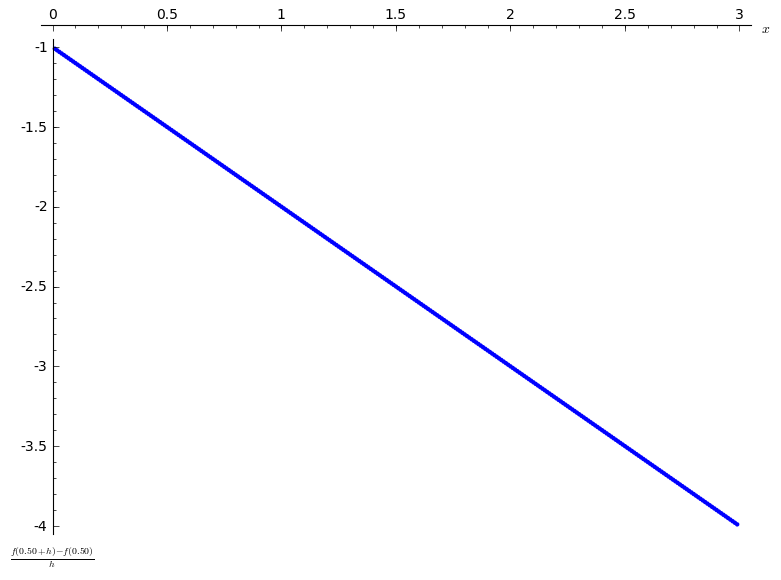
\includegraphics[width=0.9\textwidth]{illustration1.png} % first figure itself
        \caption{Convergence perf r1 r15 r1000}
    \end{minipage}\hfill
    \begin{minipage}{0.45\textwidth}
        \centering
        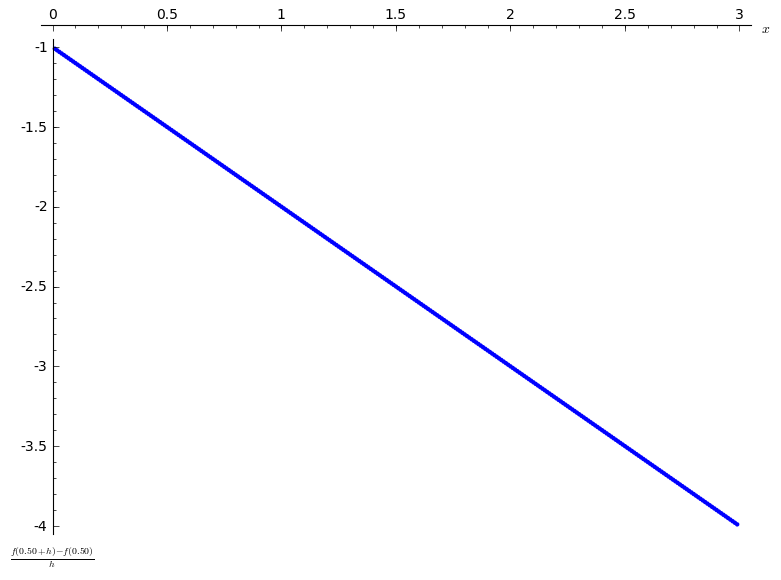
\includegraphics[width=0.9\textwidth]{illustration1.png} % second figure itself
        \caption{speed comparison}
    \end{minipage}
\end{figure}



\section{Noise robustness}
 
\begin{figure}[!ht]
    \centering
    \begin{minipage}{0.45\textwidth}
        \centering
        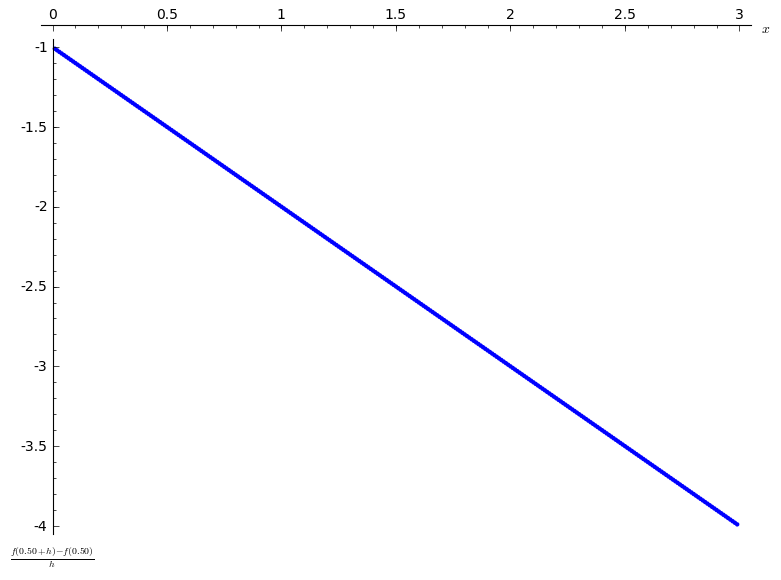
\includegraphics[width=0.9\textwidth]{illustration1.png} % first figure itself
        \caption{Perf with gaussian noise}
    \end{minipage}\hfill
    \begin{minipage}{0.45\textwidth}
        \centering
        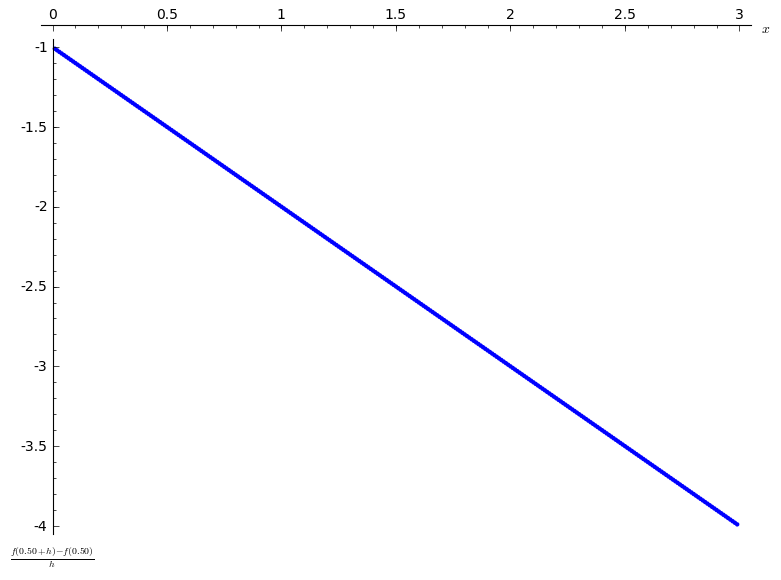
\includegraphics[width=0.9\textwidth]{illustration1.png} % second figure itself
        \caption{perf with gaussian noise and more points}
    \end{minipage}
\end{figure}

\section{Overfitting}


\begin{figure}[!ht]
    \centering
    \begin{minipage}{0.45\textwidth}
        \centering
        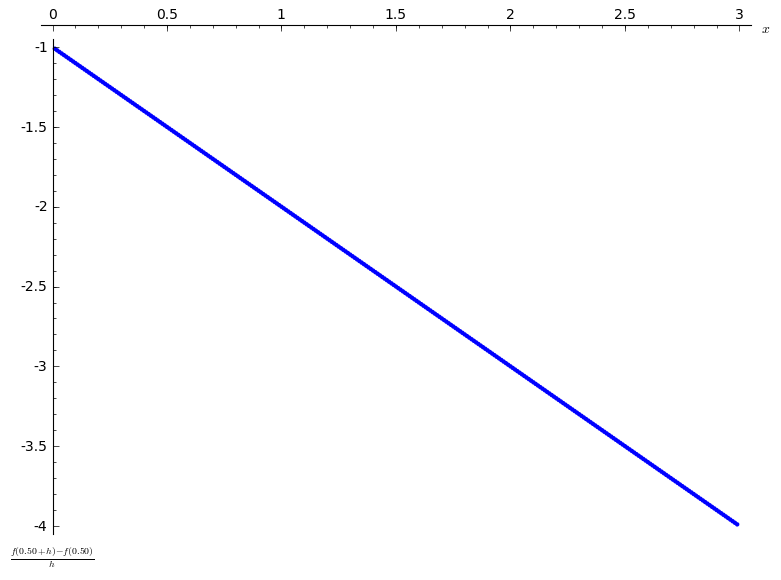
\includegraphics[width=0.9\textwidth]{illustration1.png} % first figure itself
        \caption{overfitting by  points}
    \end{minipage}\hfill
    \begin{minipage}{0.45\textwidth}
        \centering
        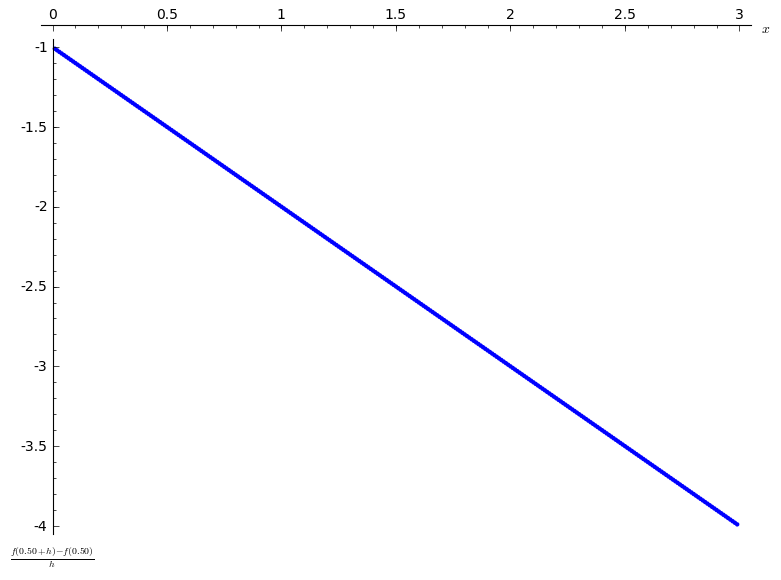
\includegraphics[width=0.9\textwidth]{illustration1.png} % second figure itself
        \caption{overfitting by  neurons}
    \end{minipage}
\end{figure}

\begin{figure}[!ht]
    \centering
    \begin{minipage}{0.45\textwidth}
        \centering
        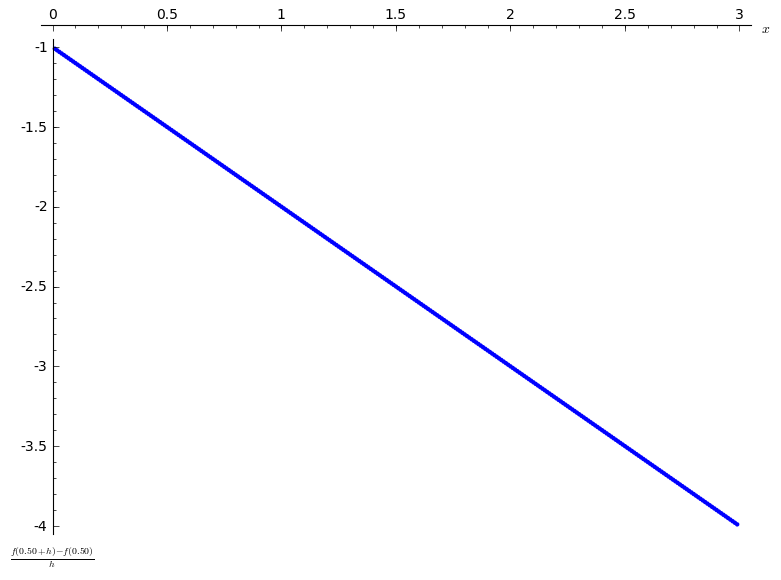
\includegraphics[width=0.9\textwidth]{illustration1.png} % first figure itself
        \caption{overfitting by  time series}
    \end{minipage}\hfill
    \begin{minipage}{0.45\textwidth}
        \centering
        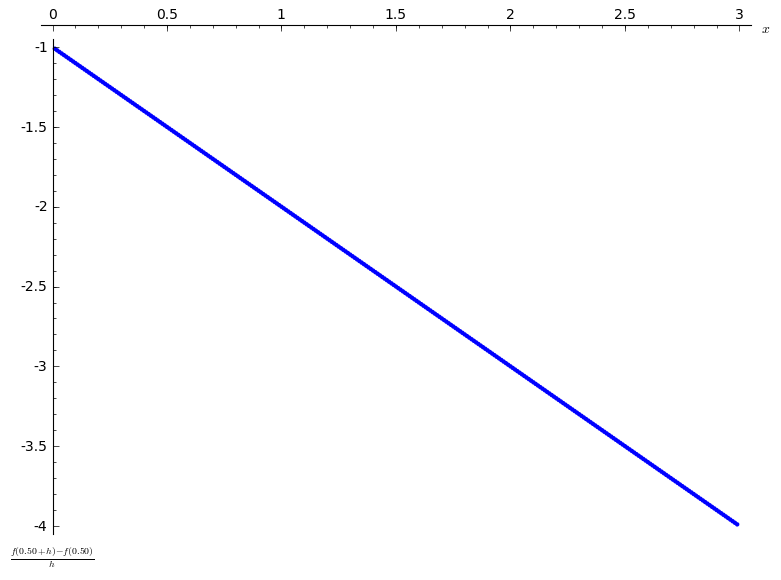
\includegraphics[width=0.9\textwidth]{illustration1.png} % second figure itself
        \caption{overfitting by  neurons}
    \end{minipage}
\end{figure}



\bibliographystyle{plain}
\bibliography{bibliography.bib}
\end{document}